%%%%%%%%%%%%%%%%%%%%%%%%%%%%%%%%%%%%%%%%%
% Jacobs Landscape Poster
% LaTeX Template
% Version 1.1 (14/06/14)
%
% Created by:
% Computational Physics and Biophysics Group, Jacobs University
% https://teamwork.jacobs-university.de:8443/confluence/display/CoPandBiG/LaTeX+Poster
% 
% Further modified by:
% Nathaniel Johnston (nathaniel@njohnston.ca)
%
% This template has been downloaded from:
% http://www.LaTeXTemplates.com
%
% License:
% CC BY-NC-SA 3.0 (http://creativecommons.org/licenses/by-nc-sa/3.0/)
%
%%%%%%%%%%%%%%%%%%%%%%%%%%%%%%%%%%%%%%%%%

%----------------------------------------------------------------------------------------
%	PACKAGES AND OTHER DOCUMENT CONFIGURATIONS
%----------------------------------------------------------------------------------------

\documentclass[final]{beamer}

\usepackage[scale=1.24]{beamerposter} % Use the beamerposter package for laying out the poster

\usetheme{confposter} % Use the confposter theme supplied with this template

\setbeamercolor{block title}{fg=ngreen,bg=white} % Colors of the block titles
\setbeamercolor{block body}{fg=black,bg=white} % Colors of the body of blocks
\setbeamercolor{block alerted title}{fg=white,bg=dblue!70} % Colors of the highlighted block titles
\setbeamercolor{block alerted body}{fg=black,bg=dblue!10} % Colors of the body of highlighted blocks
% Many more colors are available for use in beamerthemeconfposter.sty

%-----------------------------------------------------------
% Define the column widths and overall poster size
% To set effective sepwid, onecolwid and twocolwid values, first choose how many columns you want and how much separation you want between columns
% In this template, the separation width chosen is 0.024 of the paper width and a 4-column layout
% onecolwid should therefore be (1-(# of columns+1)*sepwid)/# of columns e.g. (1-(4+1)*0.024)/4 = 0.22
% Set twocolwid to be (2*onecolwid)+sepwid = 0.464
% Set threecolwid to be (3*onecolwid)+2*sepwid = 0.708

\newlength{\sepwid}
\newlength{\onecolwid}
\newlength{\twocolwid}
\newlength{\threecolwid}
\setlength{\paperwidth}{48in} % A0 width: 46.8in
\setlength{\paperheight}{36in} % A0 height: 33.1in
\setlength{\sepwid}{0.024\paperwidth} % Separation width (white space) between columns
\setlength{\onecolwid}{0.22\paperwidth} % Width of one column
\setlength{\twocolwid}{0.464\paperwidth} % Width of two columns
\setlength{\threecolwid}{0.708\paperwidth} % Width of three columns
\setlength{\topmargin}{-0.5in} % Reduce the top margin size
%-----------------------------------------------------------

\usepackage{graphicx}  % Required for including images

\usepackage{booktabs} % Top and bottom rules for tables

\usepackage{amsmath, amsthm, amssymb}
\usepackage{subfig}

%----------------------------------------------------------------------------------------
%	TITLE SECTION 
%----------------------------------------------------------------------------------------

\title{\huge{Virtual human behavioural profile extraction using Kinect based motion tracking}} % Poster title

\author{Dimitar Stanev, Konstantinos Moustakas} % Author(s)

\institute{University of Patras, Electrical and Computer Engineering Department} % Institution(s)


%----------------------------------------------------------------------------------------

\begin{document}

\addtobeamertemplate{block end}{}{\vspace*{2ex}} % White space under blocks
\addtobeamertemplate{block alerted end}{}{\vspace*{2ex}} % White space under highlighted (alert) blocks

\setlength{\belowcaptionskip}{2ex} % White space under figures
\setlength\belowdisplayshortskip{2ex} % White space under equations

\begin{frame}[t] % The whole poster is enclosed in one beamer frame

\begin{columns}[t] % The whole poster consists of three major columns, the second of which is split into two columns twice - the [t] option aligns each column's content to the top

\begin{column}{\sepwid}\end{column} % Empty spacer column

%----------------------------------------------------------------------------------------
%	FIRST COLUMN
%----------------------------------------------------------------------------------------

\begin{column}{\onecolwid}\vspace{-0.5in} % The first column

%----------------------------------------------------------------------------------------
%	OBJECTIVES
%----------------------------------------------------------------------------------------

\begin{alertblock}{Objectives}

A framework for the creation of virtual human behavioural profile which will account for physiological parameters of the body during motion activities.

\begin{itemize}
	\item Motion capture system using Kinect sensor
	\item Musculoskeletal model of the human lower extremity
	\item Generic analysis pipeline
\end{itemize}

\end{alertblock}

%----------------------------------------------------------------------------------------
%	INTRODUCTION
%----------------------------------------------------------------------------------------

\begin{block}{Introduction}

The estimation of the behavioural and physiological profile of individuals, while performing several everyday activities is a research problem related to numerous application domains ranging from physics-based modeling and simulation to computational and virtual physiological humans. Even if numerous approaches have been proposed in the past as will be analyzed in the sequel, the respective state-of-the-art is fragmented, while the use of expensive sensing equipment used reduces their application potential. The proposed framework, makes a first step towards the estimation of the behavioural and physiological profile of a human through measurements obtained from the popular Kinect sensor.

\end{block}

%----------------------------------------------------------------------------------------
%	METHODS
%----------------------------------------------------------------------------------------

\begin{block}{Methods}
	
	The motion capture system is based on the structured light sensor Kinect. The quality of capturing the human motion without noise is critical for later sages of the analysis.
	
	\begin{itemize}
		\item Full body joints tracking
		\item Moving average and threshold filters to deal with jitter noise
		\item Exponential smoothing filters for smoothing the kinematics
		\item Savitzky--Golay filter for predicting the future position and minimizing occlusion problem
	\end{itemize}

\end{block}

\end{column} % End of the first column

%----------------------------------------------------------------------------------------

%----------------------------------------------------------------------------------------
%	SECOND COLUMN
%----------------------------------------------------------------------------------------

\begin{column}{\sepwid}\end{column} % Empty spacer column

\begin{column}{\twocolwid}\vspace{-1in} % Begin a column which is two columns wide (column 2)
	
\begin{column}{\twocolwid}

	The model used for the analysis is part of the human lower extremity.
	
	\begin{itemize}
		\item Twenty degrees of freedom six for the pelvis, three rotational for the hip, one rotational for the knee, two rotational for the ankle and one rotational for the toes
		\item The model is composed of 86 muscles, where the muscle placement is based on physiological experiments
		\item The weight of the body segment is approximated based on volumetric measurements
		\item The muscle activation and contraction dynamics are based on Hill-type models
	\end{itemize}
	
	\begin{figure}[!t]
		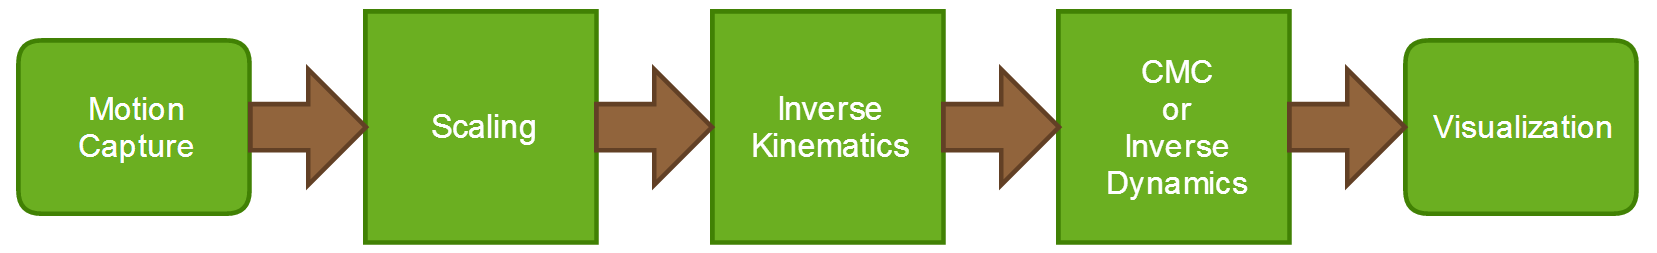
\includegraphics[width=0.85\linewidth]{fig/pipeline.png}
	\end{figure}
	
\end{column} % End of column 2.1

%----------------------------------------------------------------------------------------
%	RESULTS
%----------------------------------------------------------------------------------------

\begin{block}{Results}
	The potential of the presented framework has been investigated based on the captured motion during gait activity Figure \ref{fig:keyframe-seq}. The results show the ability of estimating the morphometrics of the subject Figure \ref{fig:kinect-mesurment}, the accuracy of the inverse kinematics Figure \ref{fig:ik-error} and the qualitative comparison between the estimated torques and the corresponding literature curves Figure \ref{fig:inverse-dynamics}.
\end{block}

%----------------------------------------------------------------------------------------
%	2 FIGURES
%----------------------------------------------------------------------------------------

\begin{columns}[t,totalwidth=\twocolwid] % Split up the two columns wide column
	
	\begin{column}{\onecolwid}\vspace{-1in}
		
		\begin{figure}[!t]
			\centering
			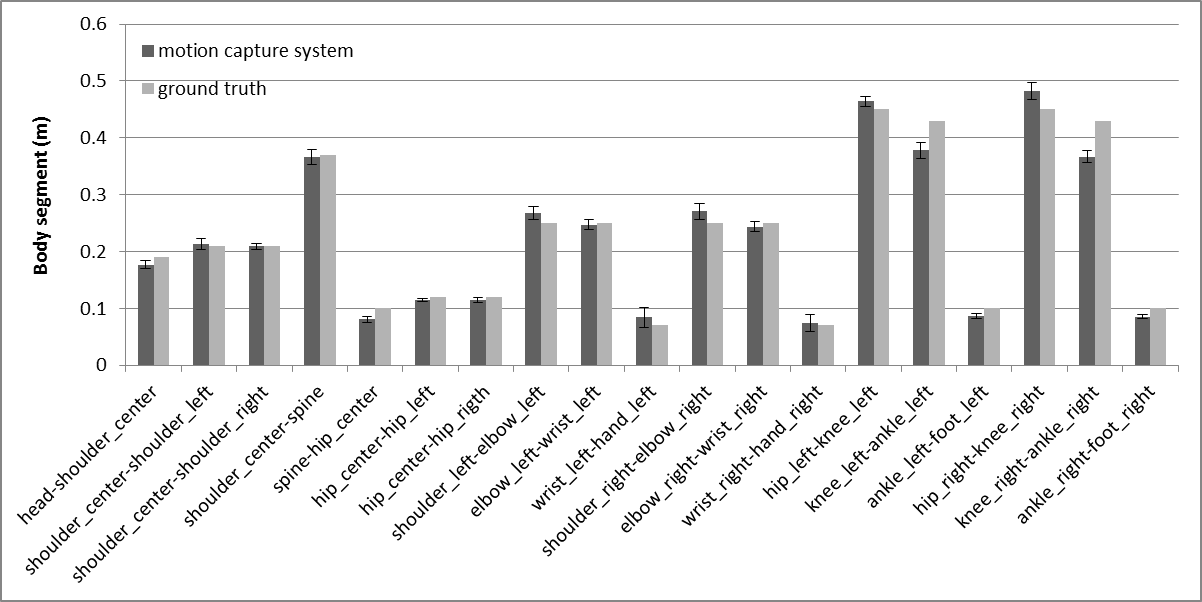
\includegraphics[width=0.95\linewidth, keepaspectratio]{fig/subject01-segments.png}
			\caption{Average length of the body with comparison to the actual lengths. The minimum and maximum standard deviation $std_{min} = 0.003m$, $std_{max} = 0.018m$ respectively.}
			\label{fig:kinect-mesurment}
		\end{figure}
		
	\end{column} % End of column 2.2
	
	\begin{column}{\onecolwid}\vspace{-1in} % The first column within column 2 (column 2.3)
		
		\begin{figure}[!t]
			\centering
			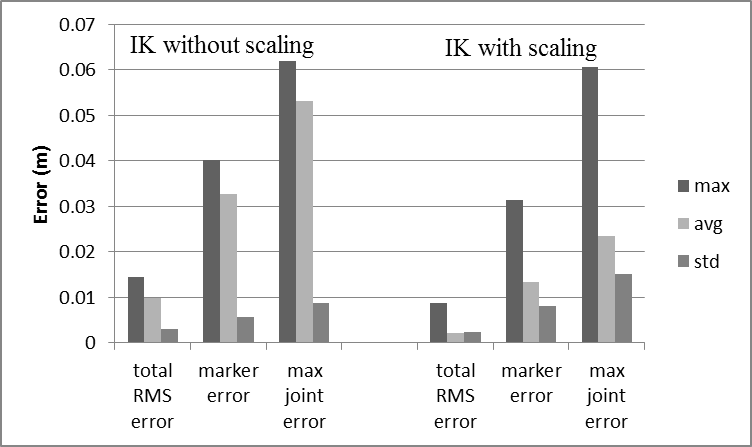
\includegraphics[width=0.8\linewidth, keepaspectratio]{fig/ik-no-scale-with-scale.png}
			\caption{Inverse kinematics errors (total RMS error, marker error, max joint error) improved after applying scaling to adjust the general model to subject's size.}
			\label{fig:ik-error}
		\end{figure}
		
	\end{column} % End of column 2.3
	
\end{columns} % End of the split of column 2

%----------------------------------------------------------------------------------------
%	INVERSE DYNAMICS
%----------------------------------------------------------------------------------------

\begin{columns}[t,totalwidth=\twocolwid] % Split up the two columns wide column again

\begin{column}{\twocolwid}

	\begin{figure}[!t]
		\centerline{
			\subfloat[Estimated hip moment]{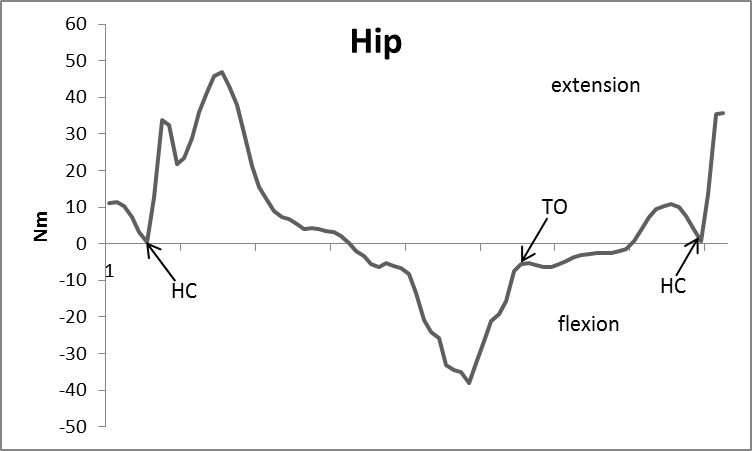
\includegraphics[width=0.3\linewidth, keepaspectratio]{fig/id-hip.png}
			\label{fig:inverse-dynamics-hip}}
			\hfil
			\subfloat[Estimated knee moment]{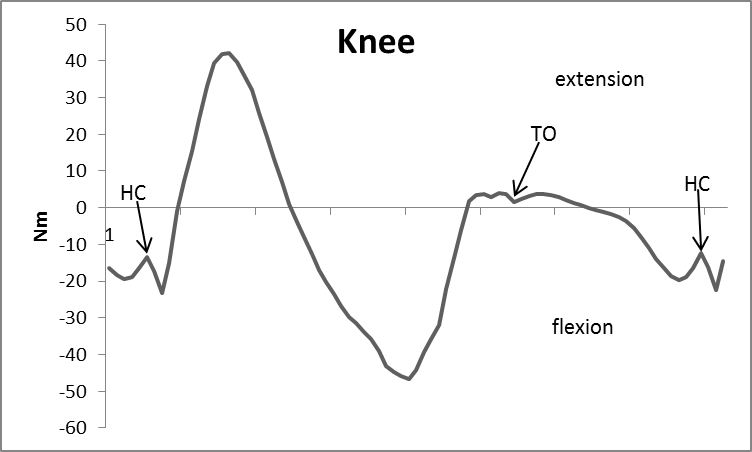
\includegraphics[width=0.3\linewidth, keepaspectratio]{fig/id-knee.png}}
			\hfil
			\subfloat[Estimated ankle moment]{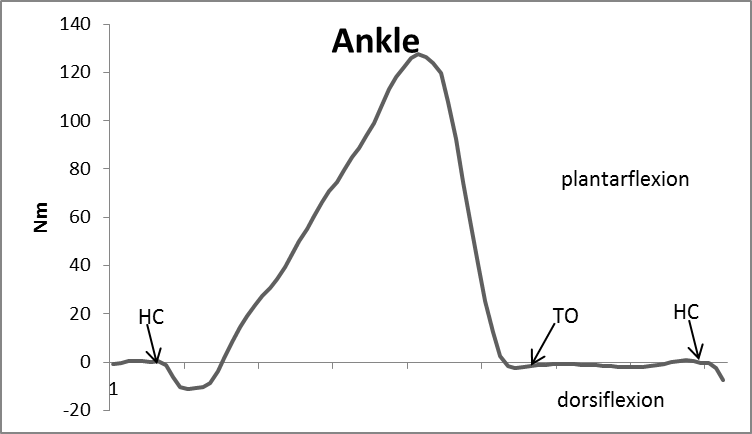
\includegraphics[width=0.3\linewidth, keepaspectratio]{fig/id-ankle.png}
			\label{fig:inverse-dynamics-ankle}}}	
		\centerline{
			\subfloat[Literature hip moment]{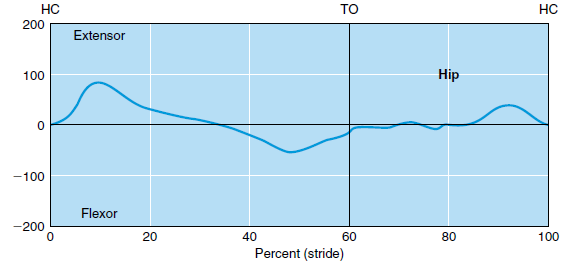
\includegraphics[width=0.33\linewidth, keepaspectratio]{fig/id-hip-ref.png}}
			\hfil
			\subfloat[Literature knee moment]{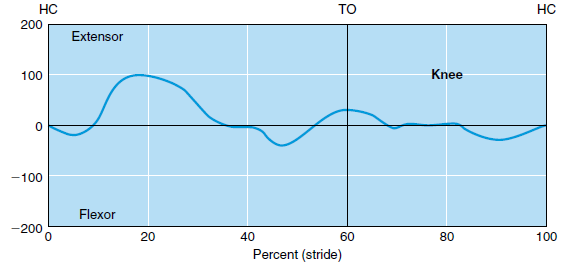
\includegraphics[width=0.33\linewidth, keepaspectratio]{fig/id-knee-ref.png}}
			\hfil
			\subfloat[Literature ankle moment]{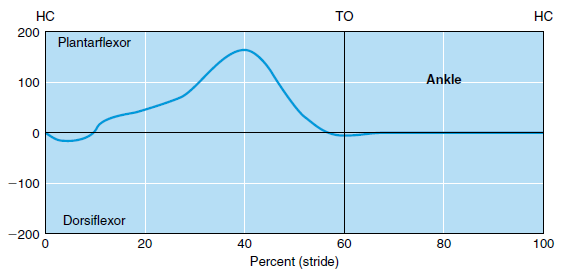
\includegraphics[width=0.33\linewidth, keepaspectratio]{fig/id-ankle-ref.png}}}
		\caption{Qualitative comparison between estimated torques (first row) and literature curves (second row) for three joints (hip, knee and ankle). Indications TO: toe off and HC: heel contact.}
		\label{fig:inverse-dynamics}
	\end{figure}

\end{column} % End of column 2.4

\end{columns} % End of the split of column 2

\end{column} % End of the second column

%----------------------------------------------------------------------------------------

\begin{column}{\sepwid}\end{column} % Empty spacer column

\begin{column}{\onecolwid}\vspace{-0.5in}% The third column
	
\begin{figure}[!t]
	\centerline{
		\subfloat[]{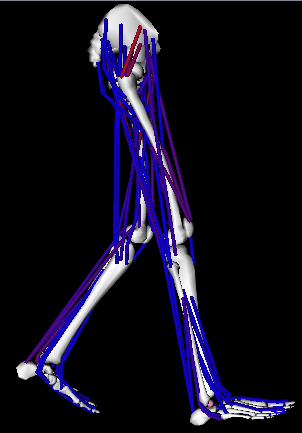
\includegraphics[width=0.25\linewidth, keepaspectratio]{fig/seq1.png}
			\label{fig:keyframe-seq-a}}
		\hfil
		\subfloat[]{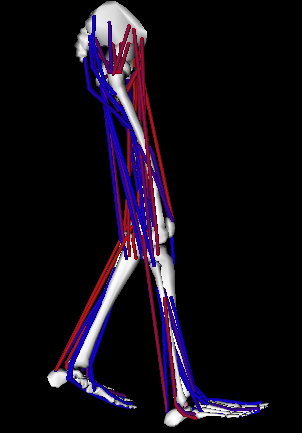
\includegraphics[width=0.25\linewidth, keepaspectratio]{fig/seq2.png}
			\label{fig:keyframe-seq-b}}
		\hfil
		\subfloat[]{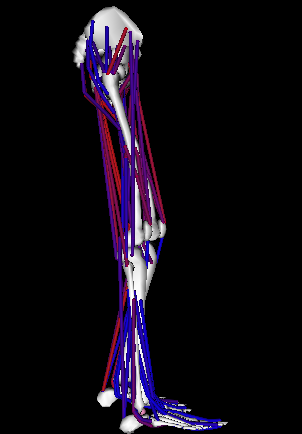
\includegraphics[width=0.25\linewidth, keepaspectratio]{fig/seq3.png}
			\label{fig:keyframe-seq-c}}
		\hfil
		\subfloat[]{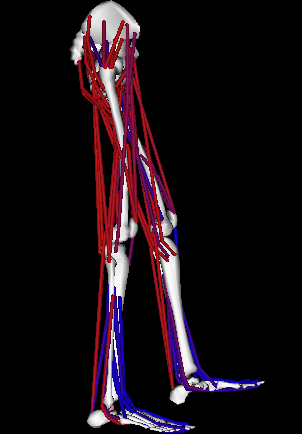
\includegraphics[width=0.25\linewidth, keepaspectratio]{fig/seq4.png}
			\label{fig:keyframe-seq-d}}}
	\caption{Key frames during gait activity with a visualization of muscle activations.}
	\label{fig:keyframe-seq}
\end{figure}

%----------------------------------------------------------------------------------------
%	CONCLUSION
%----------------------------------------------------------------------------------------

\begin{block}{Conclusion}

The major contribution of this work is based on the fact that we can reliably capture human motion activities and translate them to a virtual physiological human profile. Our approach is not limited to the motion capture system nor to the model used for analysis. Moreover, the potential applications of the proposed framework are numerous, while it is worth mentioning some of them:

\begin{itemize}
	\item The profile could be used to get personalized character animations of different characters using only a single baseline animated keyframe sequence (animation synthesis)
	\item Better and more practical disease prediction and behavioral monitoring of the patients
\end{itemize}

\end{block}


%----------------------------------------------------------------------------------------
%	REFERENCES
%----------------------------------------------------------------------------------------

%\begin{block}{References}
%
%\nocite{*} % Insert publications even if they are not cited in the poster
%\small{\bibliographystyle{unsrt}
%\bibliography{sample}\vspace{0.75in}}
%
%\end{block}

%----------------------------------------------------------------------------------------
%	ACKNOWLEDGEMENTS
%----------------------------------------------------------------------------------------

%\setbeamercolor{block title}{fg=red,bg=white} % Change the block title color

\begin{block}{Acknowledgment}
	
	This work is partially funded by the EC FP7 project NoTremor: Virtual, Physiological and Computational Neuromuscular Models for the Predictive Treatment of Parkinson's Disease, Grant Agreement No. 610391.
	
\end{block}


%----------------------------------------------------------------------------------------
%	CONTACT INFORMATION
%----------------------------------------------------------------------------------------

\setbeamercolor{block alerted title}{fg=black,bg=orange} % Change the alert block title colors
\setbeamercolor{block alerted body}{fg=black,bg=white} % Change the alert block body colors

\begin{alertblock}{Contact Information}
	
	\begin{itemize}
		\item Web: \href{www.vvr.ece.upatras.gr}{www.vvr.ece.upatras.gr}
		\item Email: \href{mailto:stanev@ece.upatras.gr}{stanev@ece.upatras.gr}
		\item Phone: +30 2610 969809
	\end{itemize}
	
\end{alertblock}

\end{column} % End of the third column

%----------------------------------------------------------------------------------------

\end{columns} % End of all the columns in the poster

\end{frame} % End of the enclosing frame

\end{document}
